\subsection{\'Etapes de validation}
\begin{frame}
  \begin{block}{Pr\'esentation}
    \begin{itemize}
      \item Tests unitaires
      \item Validation durant le programme
      \item Comparaison avec des outils existants
      \item Benchmarks
    \end{itemize}
  \end{block}
\end{frame}

\begin{frame}
\begin{figure}[H]
   \begin{minipage}[l]{.46\textwidth}
     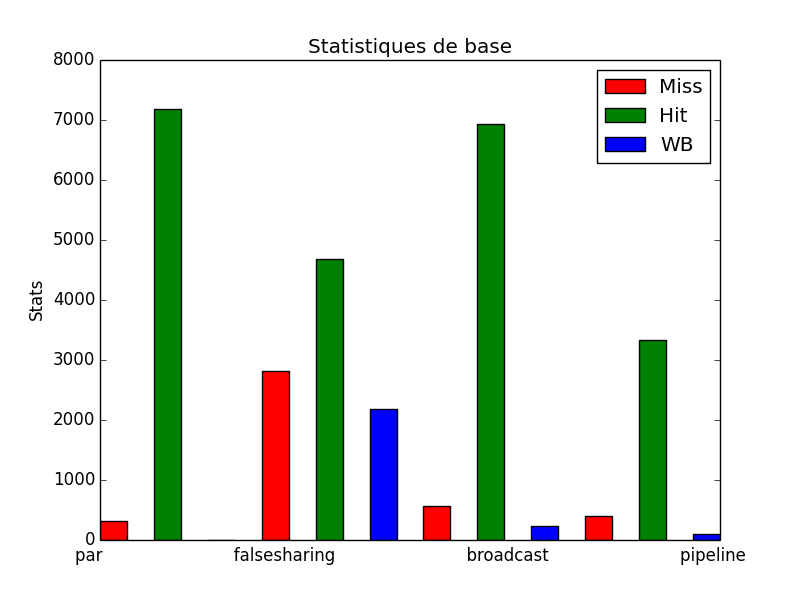
\includegraphics[scale=0.25]{images/stats_L1.png}
   \end{minipage} \hfill
   \begin{minipage}[r]{.46\textwidth}
     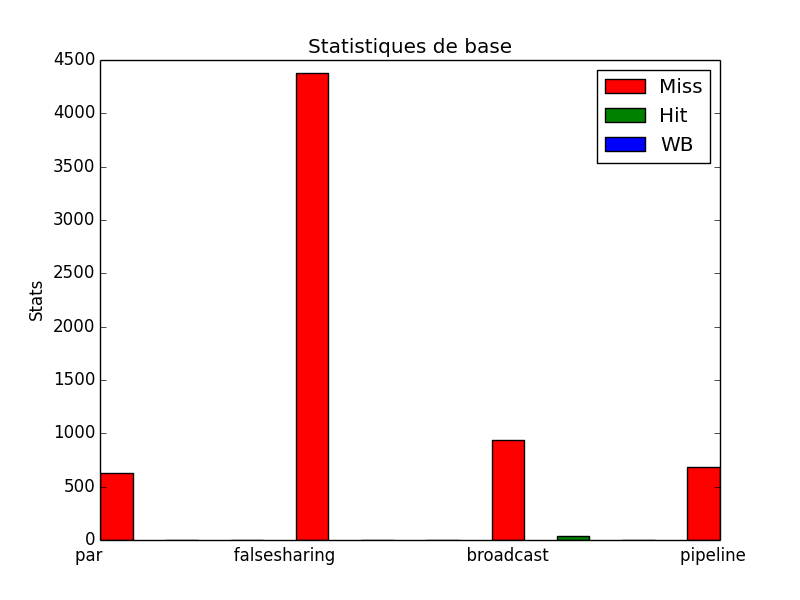
\includegraphics[scale=0.25]{images/stats_L2.png}
   \end{minipage}
\end{figure}

\begin{figure}[t!]
  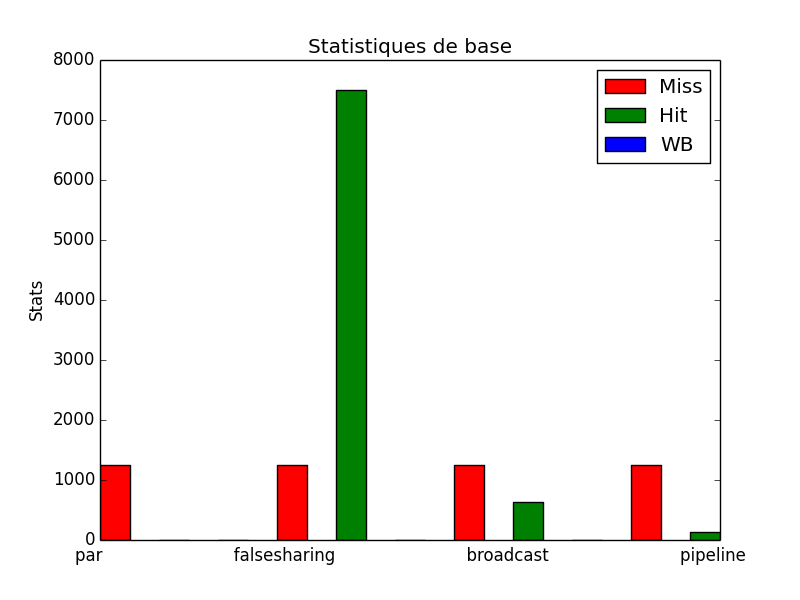
\includegraphics[width=.4\textwidth]{images/stats_L3.png}
\end{figure}
\end{frame}

\subsection{Limites \`a  propos de la simulation des caches}
\begin{frame}
  \begin{block}{Limites usuelles}
    \begin{itemize}
      \item \textsf{prefetching}
      \item synchronisations
      \item changements de contextes 
    \end{itemize}
  \end{block}
\end{frame}


\section*{Conclusion}
\begin{frame}
  \begin{block}{Objectifs atteints}
    \begin{itemize}
      \item Cahier des charges respect\'e
      \item Param\'etrisation compl\`ete
    \end{itemize}
  \end{block}

  \begin{block}{\'Evolution possible}
    \begin{itemize}
      \item Complage avec un simulateur \textsf{on-line}?
      \item Utilisation de benchmarks pour calibrer les r\'esultats?
    \end{itemize}
  \end{block}
\end{frame}
